\documentclass[10pt, landscape]{article}
\usepackage[scaled=0.92]{helvet}
\usepackage{calc}
\usepackage{multicol}
\usepackage[a4paper,margin=3mm,landscape]{geometry}
\usepackage{amsmath,amsfonts,amssymb}
\usepackage{color,graphicx,overpic}
\usepackage{hyperref}
\usepackage{newtxtext} 
\usepackage{enumitem}
\usepackage[table]{xcolor}
\usepackage{mathtools}
\usepackage{tikz}
\setlist{nosep}
% for including images
\graphicspath{ {../images/} }

\pdfinfo{
  /Title (ST2131.pdf)
  /Creator (TeX)
  /Producer (pdfTeX 1.40.0)
  /Author (Jovyn Tan)
  /Subject (ST2131)
/Keywords (ST2131, nus,cheatsheet,pdf)}

% Turn off header and footer
\pagestyle{empty}

% redefine section commands to use less space
\makeatletter
\renewcommand{\section}{\@startsection{section}{1}{0mm}%
  {-1ex plus -.5ex minus -.2ex}%
  {0.5ex plus .2ex}%x
{\normalfont\large\bfseries}}
\renewcommand{\subsection}{\@startsection{subsection}{2}{0mm}%
  {-1explus -.5ex minus -.2ex}%
  {0.5ex plus .2ex}%
{\normalfont\normalsize\bfseries}}
\renewcommand{\subsubsection}{\@startsection{subsubsection}{3}{0mm}%
  {-1ex plus -.5ex minus -.2ex}%
  {1ex plus .2ex}%
{\normalfont\small\bfseries}}%
\makeatother

\renewcommand{\familydefault}{\sfdefault}
\renewcommand\rmdefault{\sfdefault}
%  makes nested numbering (e.g. 1.1.1, 1.1.2, etc)
\renewcommand{\labelenumii}{\theenumii}
\renewcommand{\theenumii}{\theenumi.\arabic{enumii}.}
\renewcommand\labelitemii{•}
\renewcommand\labelitemiii{•}

\definecolor{mathblue}{cmyk}{1,.72,0,.38}
\everymath\expandafter{\the\everymath \color{mathblue}}

% Don't print section numbers
\setcounter{secnumdepth}{0}

%% adjust spacing for all itemize/enumerate
\setlength{\leftmargini}{0.5cm}
\setlength{\leftmarginii}{0.5cm}
\setlist[itemize,1]{leftmargin=2mm,labelindent=1mm,labelsep=1mm}
\setlist[itemize,2]{leftmargin=4mm,labelindent=1mm,labelsep=1mm}

% adding my commands
% tightcenter
\newenvironment{tightcenter}{%
  \setlength\topsep{0pt}
  \setlength\parskip{0pt}
  \begin{center}
    }{%
  \end{center}
}

% boxed
\newenvironment{tightbox}{%
  \setlength\topsep{0pt}
  \setlength\parskip{0pt}
  \begin{center}
    \begin{tabular}{|@{\hspace{\dimexpr\fboxsep+0.5\arrayrulewidth}}c@{\hspace{\dimexpr\fboxsep+0.5\arrayrulewidth}}|}
      \hline
    }
    {%
    \\ \hline
    \end{tabular}
  \end{center}
}

% fixed width box
\newenvironment{fixedbox}[1][0.7]{
  \setlength\topsep{0pt}
  \setlength\parskip{0pt}
  \begin{center}
    \begin{tabular}{|>{\centering\arraybackslash}m{#1\linewidth}|}
    \hline
  }{
  \\ \hline
  \end{tabular}
  \end{center}
}

% definition of a new term
\usepackage{soul}
\definecolor{paleyellow}{RGB}{251,243,218}
\newcommand{\definition}[2][]{\sethlcolor{paleyellow}\hl{\textbf{#2}} #1  $\rightarrow$}

% important note (attention)
\newcommand{\attention}{{\color{red}\textbf{! }}}


%  convenient absolute value symbol
\newcommand{\abs}[1]{\vert #1 \vert}

%  convenient floor and ceiling
\newcommand{\floor}[1]{\lfloor #1 \rfloor}
\newcommand{\ceil}[1]{\lceil #1 \rceil}

%  modulo with nicer spacing
\newcommand{\Mod}[1]{\ \mathrm{mod}\ #1}

%  convenient dx with nicer spacing
\newcommand{\dx}{\mathop{dx}}



% -----------------------------------------------------------------------

\begin{document}
\raggedright
\footnotesize

% space above/below equation environment 
\setlength{\abovedisplayskip}{1pt}
\setlength{\belowdisplayskip}{1pt}

\begin{multicols*}{4}
  % multicol parameters
  \setlength{\columnseprule}{0.25pt}

  \begin{center}
    \fbox{%
      \parbox{0.8\linewidth}{\centering \textcolor{black}{
          {\Large\textbf{ST2131}}
        \\ \normalsize{AY21/22 SEM 2}}
        \\ {\footnotesize \textcolor{gray}{github/jovyntls}}
      }%
    }
  \end{center}

  \section{01. COMBINATORIAL ANALYSIS}

  \textbf{factorials} - $1! = 0! = 1$

  \textbf{N1} - if we know how to count the number of different ways that an event can occur, we will know the probability of the event.

  \textbf{N2} - there are $n!$ different arrangements for $n$ objects.

  \textbf{N3} - there are $\frac{n!}{n_1!\, n_2!\, \dots n_r!}$ different arrangements of $n$ objects, 
  of which $n_1$ are alike, $n_2$ are alike, ..., $n_r$ are alike.

  \textbf{Combinations}

  \begin{tightcenter}
    $\binom{n}{r} = \frac{n!}{(n-r)!\,r!} = \binom{n-1}{r-1} + \binom{n-1}{r}, \quad 1 \leq r \leq n$
  \end{tightcenter}

  \textbf{N5} - \textbf{Binomial Theorem}: \( {\displaystyle{(x+y)^n = \sum^n_{k=0} \binom{n}{k} x^k y^{n-k} }} \) 

  \subsection{Multinomial Coefficients}

  \begin{tightcenter}
    $\binom{n}{n_1, n_2, \dots, n_r} = \frac{n!}{n_1!\, n_2!\, \dots \, n_r!}$  
  \end{tightcenter}

  \textbf{N6} - represents the number of possible divisions of $n$ distinct objects 
  into $r$ distinct groups of respective sizes $n_1, n_2, \dots, n_3$, 
  where $n_1 + n_2 + \dots + n_r = n$

  \textbf{N7} - \textbf{Multinomial Theorem}: $(x_1 + x_2 + \dots + x_r)^n=$
  \\* $\sum\limits_{(n_1, \dots, n_r):n_1 + n_2 + \dots + n_r = n} \frac{n!}{n_1! \, n_2! \, \dots n_r!} x_1^{n_1} x_2^{n_2} \dots x_r^{n_r}$

  \subsection{Number of Integer Solutions of Equations}

  \textbf{N8} - there are $\binom{n-1}{r-1}$ distinct \textit{positive} integer-valued vectors $(x_1, x_2, \dots, x_r)$ satisfying
  $x_1 + x_2 + \dots + x_r = n, \quad x_i > 0, \quad i = 1,2,\dots,r$  

  \textbf{N9} - there are $\binom{n+r-1}{r-1}$ distinct  \textit{non-negative} integer-valued vectors $(x_1, x_2, \dots, x_r)$ satisfying $x_1 + x_2 + \dots + x_r = n$ 
  \begin{niceproof}
    let $y_k = x_k + 1 \Rightarrow y_1 + y_2 + \dots + y_r = n + r$
  \end{niceproof}


  \section{02. AXIOMS OF PROBABILITY}

  \textbf{DeMorgan's Laws}: \\*
  $\mathbf{ (\bigcup\limits^n_{i=1} E_i)^c = \bigcap\limits^n_{i=1}E_i^c } \quad$ and $\quad \mathbf{ (\bigcap\limits^n_{i=1}E_i)^c = \bigcup\limits^n_{i=1}E_i^c }$ \\

  \subsection{Axioms of Probability}

  \textbf{definition 1: relative frequency}

  $P(E) = \lim_{n \to \infty} \frac{n(E)}{n}$. $\quad$ problems: (1) $\frac{n(E)}{n}$ may not converge when $n \to \infty$. (2) $\frac{n(E)}{n}$ may not converge to the same value if the experiment is repeated.

  \textbf{Axioms (definition 2)}

  For each event $E$ of the sample space $S$, we assume that a number $P(E)$ is defined and satisfies the following 3 axioms:

  1. $0 \leq P(E) \leq 1$ 
  $\quad\quad\quad\quad$
  2. $P(S) = 1$

  3. For mutually exclusive events, $P(\bigcup\limits^\infty_{i=1} E_i) = \sum\limits^\infty_{i=1} P(E_i)$. 

  \definition{mutually exclusive} $E_iE_j = \emptyset$ when  $i \neq j$

  \subsubsection{Simple Propositions}

  \textbf{N1} - $P(\emptyset) = 0$

  \textbf{N6} - \textbf{probability function} $\iff$ it satisfies the 3 axioms.

  \textbf{N8} - if $E \subset F$, then $P(E) \leq P(F)$

  \textbf{N10} - Inclusion-Exclusion identity where $n=3$
  $P(E \cup F \cup G) = P(E) + P(F) + P(G) - P(EF) - P(EG) - P(FG) + P(EFG)$

  \textbf{N11} - \textbf{Inclusion-Exclusion identity} - 

  ${\scriptstyle P(E_1 \cup E_2 \cup \dots \cup E_n) = \sum\limits^n_{i=1} P(E_i) - \sum\limits_{i_1 < i_2} P(E_{i_1} E_{i_2}) + \dots }$ 
  ${\scriptstyle + (-1)^{r+1} \sum\limits_{i_1 < \dots < i_r} P(E_{i_1} \dots E_{i_r}) + \; \dots \; + (-1)^{n+1} P(E_1 \dots E_n) }$

  \begin{enumerate}[label=(\roman*)]
    \item $P(\bigcup^n_{i=1}E_i) \leq \sum\limits^n_{i=1} P(E_i)$ 
    \item $P(\bigcup^n_{i=1}E_i) \geq \sum\limits^n_{i=1} P(E_i) - \sum\limits_{j < i} P(E_iE_j)$
  \end{enumerate}


  \subsection{Sample Space w/ Equally Likely Outcomes}

  Consider $S = \{e_1, e_2, \dots, e_n\}$. 
  Then $P(\{e_i\}) = \frac{1}{n}$ or $P(\{e_1\}) = P(\{e_2\}) = \dots = P(\{e_n\}) = \frac{1}{n}$

  \textbf{N1} - for any event $E$, $P(E) = \frac{\# \text{ of outcomes in } E}{\# \text{ of outcomes in } S}  = \frac{\# \text{ of outcomes in } E}{n} $

  \ildefinition{increasing sequence} of events $\{E_n, n \geq 1\}$ $\rightarrow$ $E_1 \subset E_2 \subset \dots \subset E_n \subset \dots$


  \ildefinition{decreasing sequence} of events $\{E_n, n \geq 1\}$ $\rightarrow$ $E_1 \supset E_2 \supset \dots \supset E_n \supset \dots$

  increasing: $\scriptstyle \lim\limits_{n \to \infty} E_n = \bigcup\limits^\infty_{i=1}E_i$, 
  decreasing: $\scriptstyle \lim\limits_{n \to \infty} E_n = \bigcap\limits^\infty_{i=1}E_i$

  \textbf{N2} - for both \textit{increasing} and \textit{decreasing} sequence, 
  $\lim\limits_{n \to \infty} P(E_n) = P(\lim\limits_{n \to \infty} E_n)$


  \section{03. CONDITIONAL PROBABILITY AND INDEPENDENCE}

  \subsection{Conditional Probability}

  \begin{tightcenter}
    if $P(F) > 0$, then $P(E|F) = \frac{P(E \cap F)}{P(F)} $

    \textbf{multiplication rule}:
    $P(E_1\dots E_n) = P(E_1)P(E_2\vert E_1)P(E_3\vert E_1 E_2) \dots P(E_n \vert E_1 E_2 \dots E_{n-1})$
  \end{tightcenter}

  \textbf{N3} - \textbf{axioms of probability} apply to conditional probability

  1.  $ 0 \leq P(E \vert F) \leq 1 $ 

  2. $ P(S \vert F) = 1 $ where $ S $ is the sample space

  3. If $ E_i $ ($ i \in \mathbb{Z}_{\geq 1} $) are mutually exclusive, then $ P(\bigcup\limits^\infty_1 E_i \vert F) = \sum\limits^\infty_1 P(E_i \vert F) $

  \textbf{N4} - If we define $ Q(E) = P(E \vert F) $, 
  then all previously proven results apply.
  \begin{itemize}
    \item $P(E_1\cup E_2\vert F ) = P(E_1\vert F ) + P(E_2\vert F ) - P(E_1 E_2\vert F ) $ 
  \end{itemize}


  \subsection{Total Probability \& Bayes' Theorem}

  \textbf{conditioning formula} - $P(E) = P(E \vert F)P(F) + P(E\vert F^c) P(F^c)$

    $P(F \vert E) = \frac{P(EF)}{P(E)} = \frac{P(F) \cdot P(E \vert F)}{P(E)}$ \\
    $P(F^c \vert E) = \frac{P(EF^c)}{P(E)} = \frac{P(F^c) \cdot P(E \vert F^c)}{P(E)}$ 

  \subsubsection{Total Probability}

  \textbf{theorem of total probability} - 
  Suppose $F_1, F_2, \dots, F_n$ are mutually exclusive events such that $\bigcup\limits^n_{i=1}F_i = S$, 
  then $P(E) = \sum\limits^n_{i=1}P(EF_i) = \sum\limits^n_{i=1}P(F_i)P(E\vert F_i)$

  \subsubsection{Bayes Theorem}
  \begin{tightcenter}
    $P(F_j \vert E) = \frac{P(EF_j)}{P(E)} = \frac{P(F_j)P(E \vert F_j)}{\sum\limits^n_{i=1} P(F_i)P(E \vert F_i)}$
  \end{tightcenter}

  \textbf{application of bayes' theorem}

  \begin{tightcenter}
    $P(B_1 \mid A) = \frac{P(A \mid B_1) \cdot P(B_1)}{P(A \mid B_1) \cdot P(B_1) + P(A \mid B_2) \cdot P(B_2)}$
  \end{tightcenter}

  Let $A$ be the event that the person test positive for a disease.
  \\* $B_1$: the person has the disease. $B_2$: does not have.
  \begin{tightcenter}
    \vspace*{-1\multicolsep}
    \begin{multicols}{2}
      true positives: $P(B_1\mid A)$
      \\ false positives: $P(A \mid B_2)$
      \\ false negatives: $P(\bar{A} \mid B_1)$
      \\ true negatives: $P(\bar{A} \mid B_2)$
    \end{multicols}
    \vspace*{-1\multicolsep}
  \end{tightcenter}

  \subsection{Independent Events}

  \textbf{N1} - $E \perp F \iff P(EF) = P(E) \cdot P(F)$ 

  \textbf{N2} - $E \perp F \iff P(E \vert F) = P(E)$

  \textbf{N3} - $E \perp F \iff E \perp F^c$ 

  \textbf{N4} - if $E, F, G$ are independent, then $E$ will be independent of any event formed from $F$ and $G$. (e.g. $F\cup G$)

  \textbf{N6} - ($ E \perp F $) $\land$ ($ E \perp G $) 
  $\not\Rightarrow $  $ E \perp FG $ 

  \textbf{N7} - For independent trials with probability $ p $ of success, probability of $ m $ successes before $ n $ failures, 
  for $ m, n \geq 1 $,

  \begin{minipage}[c]{0.3\linewidth}
    \textit{method 1}\\
    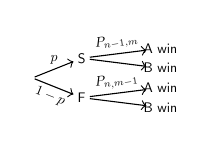
\begin{tikzpicture}[scale=0.5, every node/.style={transform shape}]
      \node[minimum size=1mm, inner sep=0] (O) at (0,1.25) {};
      \node[label=center:{S}, minimum size=4mm, inner sep=0] (S) at (1.25,1.75) {};
      \node[label=center:{F}, minimum size=4mm, inner sep=0] (F) at (1.25,0.75) {};
      \node[label=center:{A win}, minimum size=7mm, inner sep=0] (a1) at (3.25,2) {};
      \node[label=center:{B win}, minimum size=7mm, inner sep=0] (b1) at (3.25,1.5) {};
      \node[label=center:{A win}, minimum size=7mm, inner sep=0] (a2) at (3.25,1) {};
      \node[label=center:{B win}, minimum size=7mm, inner sep=0] (b2) at (3.25,0.5) {};
      \draw[->] (S) -- (a1) node[midway, above, sloped] {$P_{n-1, m}$};
      \draw[->] (S) -- (b1) node {};
      \draw[->] (F) -- (a2) node[midway, above, sloped] {$P_{n, m-1}$};
      \draw[->] (F) -- (b2) node {};
      \draw[->] (O) -- (S) node[midway, above] {$p$};
      \draw[->] (O) -- (F) node[midway, below, sloped] {$1-p$};
    \end{tikzpicture}
  \end{minipage}
  \begin{minipage}[c]{0.67\linewidth}
    \textit{method 2}

      $\scriptstyle P_{n, m} = \sum\limits^{m+n-1}_{k=n} \binom{m+n-1}{k} p^k (1-p)^{m+n-1-k}$ 

            $= P(\text{$\geq n$ successes in $ m+n-1 $ trials})$
  \end{minipage}


  \section{04. RANDOM VARIABLES}

  \subsection{Types of Random Variables}

  \begin{itemize}
    \item \definition{Bernoulli r.v.} 
      $p(x) = \begin{cases}
        p, &x=1, \text{ ('success')} \\
        1-p, &x=0\quad  \text{ ('failure')}
      \end{cases}$
    \item \definition{Binomial r.v.} $Y = X_1 + X_2 + \dots + X_n $
      where  $ X_1, X_2, \dots, X_n $ are independent Bernoulli r.v.'s.
      \begin{itemize}
        \item $ P(X=k) = \binom{n}{k} p^k (1-p)^{n-k} $
        \item $ P(k $ successes from $ n $ independent trials each with probability $ p $ of success$ ) $
      \end{itemize}
      \centerline{$E(Y) = np, \quad Var(Y) = np(1-p)$}
    \item \definition{Negative Binomial} $ X = $ \# trials until $ k $ successes
      \begin{itemize}
        \item $E[X] = k/p$
      \end{itemize}
    \item \definition{Geometric} $ X = $ number of trials until a success
      \begin{itemize}
        \item $ P(X=k) = (1-p)^{k-1} \cdot p $ where $ k $ = \# trials needed
        \item $E[X] = 1/p$
      \end{itemize}
    \item \definition{Hypergeometric} $ X = $ number of trials until success, \textit{without replacement} (for $m$ red balls of $N$ balls)
      \begin{itemize}
        \item $P(X=k) = {\binom{m}{k}\binom{N-m}{n-k}}/{\binom{N}{n}}$, $k = 0,1,\dots, n$ 
        \item $E[X] = rn/N$
      \end{itemize}
  \end{itemize}

  \subsubsection{Properties}

  \textbf{N1} - if $X \sim \text{Binomial}(n,p)$, and $Y \sim \text{Binomial}(n-1, p)$, then $E(X^k) = np \cdot E[(Y+1)^{k-1}]$

  \textbf{N2} - if $X \sim \text{Binomial}(n,p)$, then for $k \in \mathbb{Z}^+$, $P(X=k) = \frac{(n-k+1)p}{k(1-p)} \cdot P(X=k-1)$

  \subsubsection{Coupon Collector Problem}

    There are $ N $ distinct types of coupons.
    $ T $ denotes the number of coupons needed to be collected for a complete set. What is $ P(T=n) $? Ans: $ P(T>n) = \sum\limits^{N-1}_{i=1} \binom{N}{i} (\frac{N-i}{N})^n (-1)^{i+1} $

  \subsection{Probability Mass Function}

  \definition[of $X$ (\textit{discrete})]{pmf} $p(a) = P(X=a) $
  \begin{itemize}
    \item $\sum^\infty_{i=1} p(x_i) = 1$
  \end{itemize}

  \subsection{Cumulative Distribution Function}
  \begin{itemize}
    \item \definition[of a r.v. $X$]{cdf} the function $F$ defined by $\quad\quad F(x) = P(X \leq x), \quad -\infty < x < \infty$
      \begin{itemize}
        \item $F(x)$ is defined on the entire real line.
      \end{itemize}
  \end{itemize}

  \begin{minipage}[c]{0.45\linewidth}
    \begin{tightcenter}
      \textbf{pmf},
      $\begin{array}{c|ccc}
        a & 1 & 2 & 4 \\\hline
        p(a) & \frac{1}{2} & \frac{1}{4} & \frac{1}{4} 
      \end{array}$

      \ \\
      $F(a) = \sum p(x)$ for all $x \leq a$
    \end{tightcenter}
  \end{minipage}
  \begin{minipage}[c]{0.45\linewidth}
    \begin{tightcenter}
      \textbf{cdf},
      $F(a) = \begin{cases}
        0, &a < 1 \\
        1/2, &1 \leq a < 2 \\
        3/4, &2 \leq a < 4 \\
        1, &a \geq 4
      \end{cases}$
    \end{tightcenter}
  \end{minipage}

  \subsection{Expected Value, $\mu$}

  \begin{tightcenter}
    \textit{discrete}: $E(X) = \sum_x x \cdot p(x)$

    \textit{continuous}: $E(X) = \int^\infty_{-\infty} x \cdot f(x) \dx$

    $E[g(x)] = \int\limits^\infty_{-\infty} g(x) f(x) \dx $
  \end{tightcenter}

  \textbf{N1} - if $a$ and $b$ are constants, then $E(aX + b) = aE(X) + b$

  \textbf{N3} - for a non-negative r.v. $Y$, $E(Y) = \int^\infty_0 P(Y > y) \mathop{dy}$

  \begin{itemize}
    \item $I$ is an indicator variable for event $A$ if 
      $I = \begin{cases}\scriptstyle 1, \text{ if $A$ occurs} \\ \scriptstyle 0, \text{ if $A^c$ occurs}\end{cases}$. then $E(I) = P(A)$.
  \end{itemize}

  \subsubsection{2 methods for finding expectation of f(x)}

  \begin{enumerate}
    \item using pmf of $Y$: let $Y = f(X)$. Find $X$ for each $Y$.
    \item using pmf of $X$: $E[f(x)] = \sum_x f(x)p(x)$
  \end{enumerate}

  \subsection{Variance}

  For $X$ with mean $\mu = E[X]$, the \ildefinition{variance} of $X$ is 
    $Var(X) = E[(X-\mu)^2] = E(x^2) - [E(x)]^2$

  \begin{itemize}
    \item $Var(aX+b) = a^2 Var(x)$
    \item $Var(X) = \sum_{x_i} (x_i - \mu)^2 \cdot p(x_i) \quad\quad \text{(deviation $\cdot$ weight)}$
  \end{itemize}

  \subsection{Poisson Random Variable}

  $X$ is a \ildefinition{Poisson r.v.} with parameter $\lambda$ if for some $\lambda > 0$, 
  \begin{tightcenter}
    $ P(X=i) = e^{-\lambda} \cdot \frac{\lambda^i}{i!} $

    $E(X) = \lambda, \quad Var(X) = \lambda$
  \end{tightcenter}

  \begin{itemize}
    \item \textbf{Poisson Approximation of Binomial} - if $X \sim \text{Binomial}(n,p)$, where $n$ is large and $p$ is small, then $X \dot\sim \text{Poisson}(\lambda)$ where $\lambda=np$. ($\checkmark$  \textit{weak} dependence is ok) 
  \end{itemize}

  \subsection{Poisson distribution as random events}

  Let $N(t)$ be the number of events in time interval $[0, t]$. 

  \textbf{N1} - If the 3 assumptions are true, then  $N(t) \sim \text{Poisson}(\lambda t)$.

  \textbf{N2} - If $\lambda$ is the \textit{rate of occurrences} of events per unit time, then the number of occurrences in an interval of length $t$ has a Poisson distribution with mean $\lambda t$.

  \begin{tightcenter}
    $P(N(t) = k) = \frac{e^{-\lambda t} (\lambda t)^k}{k!} $, for $k \in \mathbb{Z}_{\geq 0}$
  \end{tightcenter}

  \subsubsection{o(h) notation}

  \begin{tightcenter}
    $o(h)$ stands for any function $f(h)$ such that \( {\displaystyle{ \lim_{h \to 0} \frac{f(h)}{h} = 0 }} \) 
  \end{tightcenter}

  \begin{itemize}
    \item $o(h) + o(h) = o(h)$
    \item $ \frac{\lambda t}{n} + o ( \frac{t}{n} ) \dot= \frac{\lambda t}{n} $ for large $n$
  \end{itemize}

  \subsection{Expected Value of sum of r.v.}

  For a r.v. $X$, let $X(s)$ denote the value of $X$ when $s \in \mathcal{S}$

  \textbf{N1} - $E(x) = \sum\limits_i x_i P(X=x_i) = \sum\limits_{s \in \mathcal{S}} X(s) p(s)$
  where $\mathcal{S}_i = \{s : X(s)=x_i\}$

  \textbf{N2} - $E (\sum\limits_{i-1}^n) = \sum\limits^n_{i=1}E(X_i) \quad$ for r.v. $X_1, X_2, \dots, X_n$


  \end{multicols*}

  \end{document}
